% Chapter Template

\chapter{ReactJS} % Main chapter title

\label{Chapter3} % Change 3 to a consecutive number; for referencing this chapter elsewhere, use \ref{Chapter3}

\section{Definition}
ReactJS is a JavaScript library for building web interfaces. The library was created by Jordan Walke, software engineer on Facebook, and is maintained by Facebook, Instagram and a community of individual developers and organisations. React became open source on March 2013, while it is used by Facebook since 2011, Instagram since 2012, and PayPal, Uber, Sberbank, Asana, Khan Academy, HipChat, Flipboard and Atom are a few more applications. (\cite{reactQuickly}) \par 

As mentioned in Chapter \ref{Chapter2}, library is just a set of functionalities that developers use. It doesn't aim to cover all fields of an application or to provide a complete solution for developing an app unlike frameworks. React is a UI component library which creates interactive user interfaces. It was developed for complex and large scale web based applications in order to manage how views change in response to data modifications. In that way, better user experience is provided with fast and robust development. (\cite{reactQuickly})  \par

In more details, React is mostly a view-layer solution, but it includes mechanisms for managing state without providing a specific way for data flow management, server or API interaction, or routing. For this reason, additional libraries will be needed. Its main concern is simplicity and scalability. Most popular features of React library are Virtual Document Object Model, Lifecycle Methods, Stateful components, JSX and One-way data binding that will be analyzed later on this chapter. (\cite{Reference13}) \par

\section{React Virtual DOM}

DOM stands for Document Object Model, and represents an XML or HTML document as a tree structure where each node is a different part of the document. The HTML DOM was designed for static pages and not for creating dynamic pages. So, when DOM is updated, every node and page has to be updated as well, fact that reduces application performance. For this reason, Virtual DOM was invented. Virtual DOM is basically an abstraction of HTML DOM and has analogous properties with a real DOM, with the difference that it cannot make any direct change to the screen. It is also lightweight and detached from browser and can be updated without affecting real DOM which means faster manipulation and updates. (\cite{Reference12}) \par

React differs from other front-end JavaScript frameworks, since it is not working with the browser's DOM. Alternatively, React keeps a JavaScript representation of the DOM in memory, the Virtual DOM which is a tree of JS objects, and makes all modifications in there. In that way, actual DOM is not directly manipulated and the minimum number of changes required are eventually applied to real DOM. More specifically, React compares virtual DOM with the actual one, determines which parts have been updated and then updates only those in browser's DOM. Moreover, Solutions for browser differences, server-side rendering and implementation of target rendering are provided in this way. (\cite{Reference10}) This approach brings greater performance which can be noticed by end users. (\cite{Reference13}) \par

By updating actual DOM, there are some obstacles. It is difficult to keep track of changes, the current and previous state of DOM, so as to manipulate it based on needs. Furthermore, changing the real DOM is causing low performance and high costs. For these reasons, virtual DOM was introduced which provides an API for DOM' s transformation. Developers code as if they are re-creating the whole DOM on each update. This leads to easier development model which does not require tracking changes of DOM. This implementation uses effective algorithms for rendering a JSX element so as to be aware of what has been changed and update only those elements that are modified, updates at the same time subtrees of DOM and batch the updates. (\cite{Reference10}) \par

In conclusion, React's Virtual DOM results to an easy-manipulated and improved way of building web applications. Virtual DOM is actually an intermediate area in which data are firstly changed due to faster processing. In fact, if changes in DOM are not frequent, Virtual DOM maybe is not suited, but in complex and dynamically modified ones, re-rendering whenever needed is a great feature. (\cite{Reference13}) \par

\section{Stateful Components}

React split the user interface, which is what screen shows, into smaller parts in order to be reusable and easy-maintainable. These parts are called React components and provide both data to the view and changes to it. More specifically, React is a set of components that are nested inside one another and there is one rooting component that composes all of them. Components are basically JavaScript functions that take inputs named properties and return as output React UI elements that are what is shown to the user. (\cite{Reference14})  React components include a render method that returns what has to be displayed as well as other lifecycle methods, in order code to be executed in certain times during component's life. All these methods will be described in details during next section. (\cite{Reference16}) \par

\subsection{State}
Components receive as inputs the so called "properties" that are passed externally through their parent. Except from properties, each component also have its internal state that can keep track of. (\cite{Reference13}) \par 
State is a plain JavaScript object that is used to track user events and other variables inside component.Moreover, it can be passed as properties to its child components. Furthermore, state is owned by the component, is private to it, and can be updated any time needed. Whenever component's state or its passed props are changed, the component, and all of its child components, are re-rendered. (\cite{Reference10}) \par

\section{Lifecycle Methods}

Each React component rendered into the DOM follows a series of steps. Developers can access each step through component's life-cycle methods, so tasks and specific check conditions to a stage can be performed. Lifecycle methods are used to listen changes in components. Thus, component is constant until its parent pass new props or some event causes any change in its state. (\cite{Reference13}) There are four main stages for each component's life, the so called "Mounting" stage which is the phase where an instance of a component is being created and inserted into DOM, the "Updating" which is the phase where component is being re-rendered, the "Unmounting" where component is being deleted from the DOM, and another not that critical, the "Error Handling" for any errors occurred during rendering. Each of first three previously mentioned stages of component's life include their own methods that will be described in details. (\cite{Reference16})  \par

Before a component has been placed into DOM for first time, a method named \textbf{componentWillMount} is applied so as component to receive timers and data needed from the server. Method \textbf{constructor}  belongs to "Mounting" stage and is called when initializing the component. In this stage \textbf{render} method is also called and converts JSX elements to HTML which place them into DOM, or in other words mounts component. After mounting is done, method \textbf{componentDidMount} is called and used as an integration between non-React and React libraries. (\cite{Reference13}) \par

The first method called when either props or state has been changed, or in other words during the "Updating" stage, is \textbf{shouldComponentUpdate}. The method receives two arguments a new set of properties and a new state, and compares those with the old ones. Moreover, this method is returning a boolean value. (\cite{Reference13}) If the value returned is false, then the update is aborted which means that the render method won't be invoked, while if it is true, the update is normally happening. This is useful for performance reasons of the application, only in cases that the changes made are not that necessary to be made. Rendering is generally considered as computationally expensive and can slow down the application. This decision is made based on either the comparison of new and old state and properties, or if the component is static and doesn't need to be re-rendered. (\cite{Reference14}) If method is not defined, its default value is true. The next method called, if the previously mentioned method return true, is \textbf{render} again. In this case, render gets the new JSX representations, compares it to the old one into the virtual DOM, and creates and apply changed parts to real DOM. Finally, once this process is complete, \textbf{componentDidUpdate} which receives the previous state and properties as arguments is executed. This is used to operate on the DOM, like doing network requests, after component has been updated. (\cite{Reference16}) After that the update lifecycle, the components remains inactive until a change to be occurred. This methods are executed all over again unless the component is unmounted from DOM. (\cite{Reference13}) \par 

As regards the "Unmounting" stage, there is only one method called named textbf{componentWillUnmount} which does not receive any arguments. This method is executed right before the component is removed from DOM and is the final stage of component's life. (\cite{Reference14}) In this phase, any necessary cleanup is performed. Anything that has been created over component's lifecycle, such as invalidating timers, canceling network requests, or cleaning up subscriptions made, are removed through this method. (\cite{Reference16}) \par 

Each of the methods mentioned above might be used inside a component, but their usage is optional and based on component's functionality needs. Furthermore, it is a good practice to use these methods for DOM manipulation and not other kind of libraries alongside React. This is because React uses a virtual representation of DOM in order to apply and manage changes in browser's DOM. So, if other libraries are used, there are possibilities of not being synchronized with React expectations so as errors to happen when React tries to match changes. (\cite{Reference13}) \par

\section{JSX}

JSX, which stands for "JavaScript XML", was created by Facebook community for React library and it is an extension to ESCMAScript syntax. ECMAScript or ES is a standard formation body of JS scripting language, as referred to Chapter \ref{Chapter2}, and the ES6 version is mostly used among JavaScript developers. More specifically, JSX has a syntax analogous to HTML and is a markup language compiled to ES6 that aims to define component's layout. It is not necessary to be used alongside with React, but is considered as good practice, otherwise React is becoming much more complex and with lower performance. Furthermore, JSX includes tools for converting ES6 to ES5, the browser-compatible syntax. (\cite{Reference13}) \par

JSX describes the way user interface should look like by producing React elements. Events handler, state changes and data represented are closely related to UI logic. For this reason, JSX's components contain both markup and logic-based technologies in the same file, fact that differentiates React from other frameworks or libraries.(\cite{Reference16}) In that way, a lot useful errors and warnings are being caught because of the debugging made during compilation process.(\cite{Reference10}) Another benefit of JSX is the speed. Even if JSX is compiled to JS, its output is optimized with a better way compared to the same code written directly in JavaScript. In mobile applications has been found that JSX is 12 \% faster in IOS and 29 \% in Androids than pure JS code. (\cite{Reference14}) To sum up, JSX is a representation of component's HTML in JS and also close to object-oriented languages, like Java. (\cite{Reference13})

\subsection{Babel}

As referred in Chapter \ref{Chapter2}, nowadays the majority of browsers do not support ES6 or other languages, except ES5. This is happening because it takes time to update JavaScript engines of browsers and much more time for users to upgrade to their latest version. So, any language used in client side needs to be converted to ES5 so as this gap to be closed and code to be executed in any browser.(\cite{Reference10}) For this purpose, there are two main compilers, traceur32 by Google and babel33 by JavaScript community. These two are not used for Typescript transition to browser-compatible code, but for pure ES6 code. (\cite{murray2018ng})

As regards Babel, or babel133, is a JavaScript transpiler that changes ES6 to ES5 code as it has been pointed out. However, this tranpiller includes the ability to understand JSX. In this way, JSX can be compiled to conventional ES5 and browser to normally execute code.  (\cite{Reference10})

\section{One-way data binding}
 
Data binding is the way connection between user interface and business logic is succeeded. When binding of these two layers is properly built, components, that are connected to recently modified data, are re-rendered. (\cite{Reference21}) There are three main types of binding, one-way binding, two-way binding and Observables, as it is analyzed in Chapter \ref{Chapter2}. \par

React follows one-way data flow which means state can change view, but not vice versa. One-way flow or binding is an one-way direction from state to view that keeps under control state and models, and makes application's architecture less complex and more predictable. Data pass only from parent to child components, so in case changes are made, event handlers need to be emitted. Even if it is needed extra code for setting data through event handlers to state in order view to be rendered, complex user interface and the amount of views and states needed are reduced in a large extend. (\cite{reactQuickly}) \par

Generally, This way of binding is suitable for applications that do not need to control view's changes. (\cite{Reference21}) React combined with Redux so as one-way binding to be provided. \par

\subsection{Redux}

React is well combined with Redux since one-way data flow pattern is adopted, as figure 3.2 also reveals. Redux is providing data management and a global store to the application which leads to scalability and interactivity. Any data can be updated from any view at anytime and, in this way, debugging is easier. A lot services are using Redux alongside with React for faster responses and a better user experience, such as Facebook, Instagram and Airbnb (\cite{Reference12})

The process when using Redux is shown in figure 3.1 bellow. When a user interacts with the application, an action related to this interaction is dispatched. In case an HTTP request is required to server side, the action is returned and awaits for the response. Action and current state are sent to reducer when request to server is fulfilled, and reducer creates the new state and substitutes the old one. Finally, any component, that its state has been changed based on the updates in store, is re-rendered. (\citeyearpar{murray2018ng})

\begin{figure}[h!]
	\begin{center}
		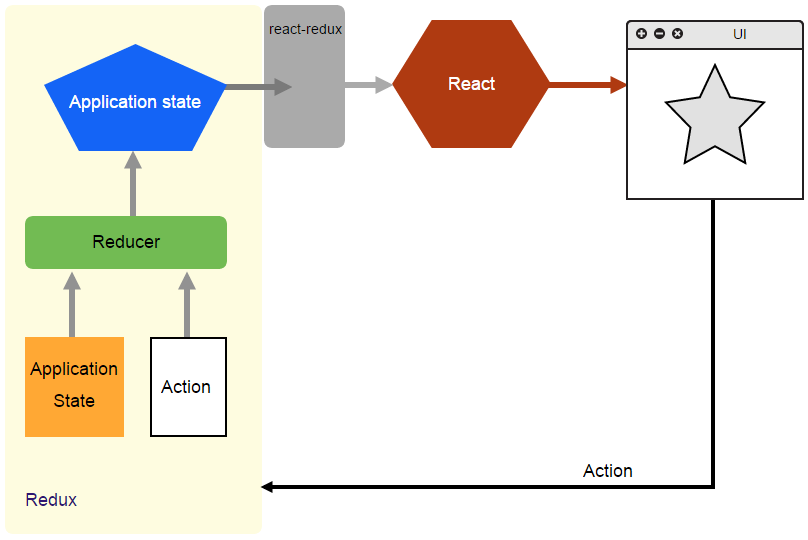
\includegraphics[scale=0.3]{images/Redux.png}
	\end{center}
	\caption{React with Redux}
\end{figure}

\section{Summery}

React library has changed the way user interface is developed by building stateful components in JSX syntax. React is one of the most popular libraries between front-end developers and well-known companies for client side layer. In this chapter, was covered the definition and conceptual fundamentals of React, as well as some external libraries used for its better usage. \par

% 6 pages
